\section{拥塞控制引擎}
\label{sec:congestion_control_engine}
在Linux中,实现了多种不同的拥塞控制算法。为了简化拥塞控制算法的编写,Linux的开发
者们实现了一套拥塞控制引擎或者说是框架,专门用于实现拥塞控制算法。只要实现必要的
接口,即可完成一套拥塞控制算法,极大地简化了拥塞控制算法的开发工作。

\subsection{接口}
\label{subsec:congestion_control_interface}

\subsubsection{\mintinline{c}{tcp_congestion_ops}}
\mintinline{c}{struct tcp_congestion_ops}结构体描述了一套拥塞控制算法所需要
支持的操作。其原型如下:
\begin{minted}[linenos]{c}
/*
Location

	include/net/tcp.h
*/
struct tcp_congestion_ops {
		/*链接注册到系统中不同的各种拥塞算法*/
        struct list_head        list;
        u32 key; /* 算法名称的哈希值 */
        u32 flags;

        /* 初始化私有数据 (可选) */
        void (*init)(struct sock *sk);
        /* 释放私有数据  (可选) 
			调用场合:
				1.关闭套接口
				2.传输控制块选择了另一种拥塞控制算法
		*/
        void (*release)(struct sock *sk);

        /* 返回ssthresh (必须实现) */
        u32 (*ssthresh)(struct sock *sk);
        /* 计算新的拥塞窗口 (必须实现) */
        void (*cong_avoid)(struct sock *sk, u32 ack, u32 acked);
        /* 在改变ca_state前会被调用 (可选) */
        void (*set_state)(struct sock *sk, u8 new_state);
        /* 处理拥塞窗口相关的事件 (可选) */
        void (*cwnd_event)(struct sock *sk, enum tcp_ca_event ev);
        /* 处理ACK包到达事件 (可选) */
        void (*in_ack_event)(struct sock *sk, u32 flags);
        /* 用于撤销“缩小拥塞窗口” (可选) */
        u32  (*undo_cwnd)(struct sock *sk);
        /* 有段被确认时会调用此函数 (可选)
			num_acked为此次ACK确认的段数
		 */
        void (*pkts_acked)(struct sock *sk, u32 num_acked, s32 rtt_us);
        /* 为inet_diag准备的获取信息的接口 (可选) */
        size_t (*get_info)(struct sock *sk, u32 ext, int *attr,
                           union tcp_cc_info *info);

        /* 拥塞控制算法的名称 */
        char            name[TCP_CA_NAME_MAX];
        struct module   *owner;
};
\end{minted}

		\subsubsection{拥塞控制事件}
			为了将拥塞控制算法相关的部分抽取处理,Linux的开发者们采用了事件机制,即在发生和拥塞控制
			相关的事件后,调用拥塞控制算法中的事件处理函数,以通知拥塞控制模块,具体发生了什么。
			而作为实现拥塞控制算法的开发者,则无需关心事件是如何发生的,以及相关的实现,只要
			专注于事件所对应的需要执行的算法即可。

			当发生相关事件是会调用\mintinline{c}{cwnd_event}函数。该函数会传入一个枚举值作为参数,
			代表具体发生的事件。该枚举值的定义如下:
\begin{minted}[linenos]{c}
/*
Location

	include/net/tcp.h
*/
enum tcp_ca_event {
        /* 首次传输,且无已发出但还未确认的包 */
        CA_EVENT_TX_START,
        /* 拥塞窗口重启 */
        CA_EVENT_CWND_RESTART,  
        /* 拥塞恢复结束 */
        CA_EVENT_COMPLETE_CWR,
        /* 超时,进入loss状态 */
        CA_EVENT_LOSS,          
        /* ECN 被设置了,但 CE 没有被置位 */
        CA_EVENT_ECN_NO_CE,     
        /* 收到了设置了 CE 位的IP报文 */
        CA_EVENT_ECN_IS_CE,     
        /* 延迟确认已被发送 */
        CA_EVENT_DELAYED_ACK,
        CA_EVENT_NON_DELAYED_ACK,
};
\end{minted}

当收到了ACK包时,会调用\mintinline{c}{in_ack_event()}。此时也会传递一些信息给拥塞
控制算法。相关的定义如下:
\begin{minted}[linenos]{c}
enum tcp_ca_ack_event_flags {
        CA_ACK_SLOWPATH         = (1 << 0),     /* 在慢速路径中处理 */
        CA_ACK_WIN_UPDATE       = (1 << 1),     /* 该ACK更新了窗口大小 */
        CA_ACK_ECE              = (1 << 2),     /* ECE 位被设置了 */
};
\end{minted}


		\subsubsection{\mintinline{c}{tcp_register_congestion_control()}}
			该函数用于注册一个新的拥塞控制算法。
\begin{minted}[linenos]{c}
int tcp_register_congestion_control(struct tcp_congestion_ops *ca)
{
        int ret = 0;

        /* 所有的算法都必须实现 ssthresh 和 cong_avoid ops */
        if (!ca->ssthresh || !ca->cong_avoid) {
                pr_err("%s does not implement required ops\n", ca->name);
                /* 如果没实现,则返回错误 */
                return -EINVAL;
        }

        /* 计算算法名称的哈希值,加快比对速度。 */
        ca->key = jhash(ca->name, sizeof(ca->name), strlen(ca->name));

        spin_lock(&tcp_cong_list_lock);
        if (ca->key == TCP_CA_UNSPEC || tcp_ca_find_key(ca->key)) {
                /* 如果已经注册被注册过了,或者恰巧hash值重了(极低概率),
                 * 那么返回错误值。
                 */
                pr_notice("%s already registered or non-unique key\n",
                          ca->name);
                ret = -EEXIST;
        } else {
                /* 将算法添加到链表中 */
                list_add_tail_rcu(&ca->list, &tcp_cong_list);
                pr_debug("%s registered\n", ca->name);
        }
        spin_unlock(&tcp_cong_list_lock);

        return ret;
}
\end{minted}
	其中,\mintinline{c}{tcp_ca_find_key}函数通过哈希值来查找名称。jash是一种久经考验的
	性能极佳的哈希算法。据称,其计算速度和产生的分布都很漂亮。这里计算哈希值正是使用了这种
	哈希算法。早些版本的内核查找拥塞控制算法,是通过名字直接查找的,如下:
\begin{minted}[linenos]{c}
/* Simple linear search, don't expect many entries! */
static struct tcp_congestion_ops *tcp_ca_find(const char *name)
{
        struct tcp_congestion_ops *e;

        list_for_each_entry_rcu(e, &tcp_cong_list, list) {
                if (strcmp(e->name, name) == 0)
                        return e;
        }

        return NULL;
}
\end{minted}
	可以看到,每次查找都要对比字符串,效率较低。这里为了加快查找速度,对名字进行了哈希,
	并通过哈希值的比对来进行查找。
\begin{minted}[linenos]{c}
/* Simple linear search, not much in here. */
struct tcp_congestion_ops *tcp_ca_find_key(u32 key)
{
        struct tcp_congestion_ops *e;

        list_for_each_entry_rcu(e, &tcp_cong_list, list) {
                if (e->key == key)
                        return e;
        }

        return NULL;
}
\end{minted}
	一般情况下,拥塞控制算法都作为单独的模块实现。以便于更加方便地使用。在模块初始化时,调用
	\mintinline{c}{tcp_register_congestion_control}函数来进行注册,
	之后,即可使用新的拥塞控制算法。

		\subsubsection{\mintinline{c}{tcp_unregister_congestion_control()}}
			与注册相对应的,
			\mintinline{c}{tcp_unregister_congestion_control}用于撤销一个拥塞控制算法。
			其实现如下:
\begin{minted}[linenos]{c}
void tcp_unregister_congestion_control(struct tcp_congestion_ops *ca)
{
        spin_lock(&tcp_cong_list_lock);
        /* 删除该拥塞控制算法 */
        list_del_rcu(&ca->list);
        spin_unlock(&tcp_cong_list_lock);

        /* Wait for outstanding readers to complete before the
         * module gets removed entirely.
         *
         * A try_module_get() should fail by now as our module is
         * in "going" state since no refs are held anymore and
         * module_exit() handler being called.
         */
        synchronize_rcu();
}
\end{minted}

	\subsection{CUBIC拥塞控制算法}
		Cubic算法是Linux中默认的拥塞控制算法。

			\subsubsection{CUBIC算法介绍}
				CUBIC算法的思路是这样的:当发生了一次丢包后,它将此时的窗口大小定义为$W_{max}$,之后,
				进行乘法减小。这里与标准TCP不同,乘法减小时不是直接减小一半,而是乘一个常系数$\beta$。
				快重传和快恢复的部分和标准TCP一致。当它进入到拥塞避免阶段以后,它根据cubic函数凹的部分
				进行窗口的增长,直至到达$W_{max}$为止。之后,它会根据cubic函数凸的部分继续增长。

\begin{figure}[htpb]
\centering
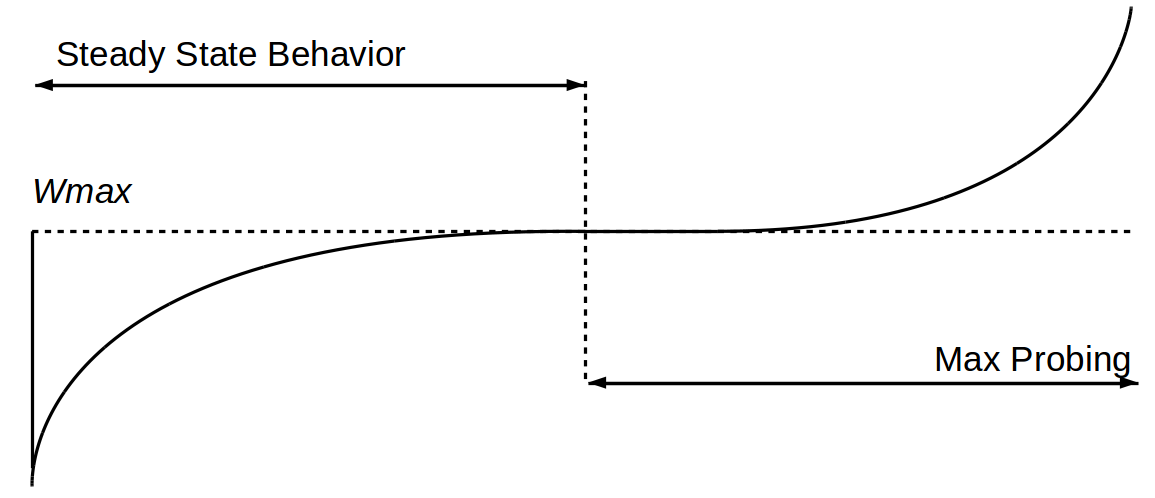
\includegraphics[width=\textwidth]  {images/cubic.png}
\caption{Cubic函数}
\end{figure}

\subsubsection{模块定义}
在Linux中,拥塞控制算法是作为模块单独实现的。Cubic也不例外。首先,定义了模块的基本信息
\begin{minted}[linenos]{c}
module_init(cubictcp_register);
module_exit(cubictcp_unregister);

MODULE_AUTHOR("Sangtae Ha, Stephen Hemminger");
MODULE_LICENSE("GPL");
MODULE_DESCRIPTION("CUBIC TCP");
MODULE_VERSION("2.3");
\end{minted}
这部分定义包括了模块作者、所使用的许可证、版本等等。其中,最重要的是定义了模块的初始化函数,
和模块被卸载时所要调用的函数。初始化函数如下:
\begin{minted}[linenos]{c}
static int __init cubictcp_register(void)
{       
        BUILD_BUG_ON(sizeof(struct bictcp) > ICSK_CA_PRIV_SIZE);
        
        /* 预先计算缩放因子(此时假定SRTT为100ms) */
        
        beta_scale = 8*(BICTCP_BETA_SCALE+beta) / 3
                / (BICTCP_BETA_SCALE - beta);
        
        cube_rtt_scale = (bic_scale * 10);      /* 1024*c/rtt */
        
        /* 计算公式 (wmax-cwnd) = c/rtt * K^3 中的K
         * 可得 K = cubic_root( (wmax-cwnd)*rtt/c )
         * 注意,这里 K 的单位是 bictcp_HZ=2^10, 而不是 HZ
         */
        
        /* 1/c * 2^2*bictcp_HZ * srtt */
        cube_factor = 1ull << (10+3*BICTCP_HZ); /* 2^40 */
        
        /* divide by bic_scale and by constant Srtt (100ms) */
        do_div(cube_factor, bic_scale * 10);
        
        return tcp_register_congestion_control(&cubictcp);
}
\end{minted}
在初始化时,根据预先设定好的参数,按照Cubic算法的公式计算好\mintinline{c}{cube_factor}。
之后,调用\mintinline{c}{tcp_register_congestion_control}函数注册Cubic算法。
Cubic算法所实现的操作如下:
\begin{minted}[linenos]{c}
static struct tcp_congestion_ops cubictcp __read_mostly = {
        .init           = bictcp_init,
        .ssthresh       = bictcp_recalc_ssthresh,
        .cong_avoid     = bictcp_cong_avoid,
        .set_state      = bictcp_state,
        .undo_cwnd      = bictcp_undo_cwnd,
        .cwnd_event     = bictcp_cwnd_event,
        .pkts_acked     = bictcp_acked,
        .owner          = THIS_MODULE,
        .name           = "cubic",
};
\end{minted}
根据这里定义好的操作,我们就可以去理解对应的实现。在模块被卸载时,
将调用\mintinline{c}{cubictcp_unregister}函数。该函数只有一个职责——将Cubic算法
从拥塞控制引擎中注销掉。
\begin{minted}[linenos]{c}
static void __exit cubictcp_unregister(void)
{
        tcp_unregister_congestion_control(&cubictcp);
}
\end{minted}

\subsubsection{基本参数及初始化}
CUBIC的所需的基本参数定义如下:
\begin{minted}[linenos]{c}
/* BIC TCP Parameters */
struct bictcp {
        u32     cnt;            /* 每次cwnd增长1/cnt的比例 */
        u32     last_max_cwnd;  /* snd_cwnd之前的最大值 */
        u32     loss_cwnd;      /* 最近一次发生丢失的时候的拥塞窗口 */
        u32     last_cwnd;      /* 最近的snd_cwnd */
        u32     last_time;      /* 更新last_cwnd的时间 */
        u32     bic_origin_point;/* bic函数的初始点 */
        u32     bic_K;          /* 从当前一轮开始到初始点的时间 */
        u32     delay_min;      /* 最小延迟 (msec << 3) */
        u32     epoch_start;    /* 一轮的开始 */
        u32     ack_cnt;        /* ack 的数量 */
        u32     tcp_cwnd;       /* estimated tcp cwnd */
        u16     unused;
        u8      sample_cnt;     /* 用于决定curr_rtt的样本数 */
        u8      found;          /* 是否找到了退出点? */
        u32     round_start;    /* beginning of each round */
        u32     end_seq;        /* end_seq of the round */
        u32     last_ack;       /* last time when the ACK spacing is close */
        u32     curr_rtt;       /* the minimum rtt of current round */
};
\end{minted}

初始化时,首先重置了CUBIC所需的参数,之后,将\mintinline{c}{loss_cwnd}设置为0。
因为此时尚未发送任何丢失,所以初始化为0。最后根据是否启用hystart机制来决定是否进行相应的
初始化。最后,如果设置了\mintinline{c}{initial_ssthresh},那么就用该值作为初始的
\mintinline{c}{snd_ssthresh}。
\begin{minted}[linenos]{c}
static void bictcp_init(struct sock *sk)
{
        struct bictcp *ca = inet_csk_ca(sk);

        bictcp_reset(ca);
        ca->loss_cwnd = 0;

        if (hystart)
                bictcp_hystart_reset(sk);

        if (!hystart && initial_ssthresh)
                tcp_sk(sk)->snd_ssthresh = initial_ssthresh;
}
\end{minted}
其中,\mintinline{c}{bictcp_reset}函数将必要的参数都初始化为0了。
\begin{minted}[linenos]{c}
static inline void bictcp_reset(struct bictcp *ca)
{
        ca->cnt = 0;
        ca->last_max_cwnd = 0;
        ca->last_cwnd = 0;
        ca->last_time = 0;
        ca->bic_origin_point = 0;
        ca->bic_K = 0;
        ca->delay_min = 0;
        ca->epoch_start = 0;
        ca->ack_cnt = 0;
        ca->tcp_cwnd = 0;
        ca->found = 0;
}
\end{minted}

\subsubsection{ssthresh的计算}
门限值的计算过程在\mintinline{c}{bictcp_recalc_ssthresh}函数中实现。
\begin{minted}[linenos]{c}
static u32 bictcp_recalc_ssthresh(struct sock *sk)
{
        const struct tcp_sock *tp = tcp_sk(sk);
        struct bictcp *ca = inet_csk_ca(sk);

        ca->epoch_start = 0;    /* end of epoch */

        /* Wmax and fast convergence */
        if (tp->snd_cwnd < ca->last_max_cwnd && fast_convergence)
                ca->last_max_cwnd = (tp->snd_cwnd * (BICTCP_BETA_SCALE + beta))
                        / (2 * BICTCP_BETA_SCALE);
        else
                ca->last_max_cwnd = tp->snd_cwnd;

        ca->loss_cwnd = tp->snd_cwnd;

        return max((tp->snd_cwnd * beta) / BICTCP_BETA_SCALE, 2U);
}
\end{minted}
这里涉及到了Fast Convergence机制。该机制的存在是为了加快CUBIC算法的收敛速度。
在网络中,一个新的流的加入,会使得旧的流让出一定的带宽,以便给新的流让出一定的增长空间。
为了增加旧的流释放的带宽量,CUBIC的作者引入了Fast Convergence机制。每次发生丢包后,
会对比此次丢包时拥塞窗口的大小和之前的拥塞窗口大小。如果小于了之前拥塞窗口的最大值,
那么就说明可能是有新的流加入了。此时,就多留出一些带宽给新的流使用,以使得网络尽快
收敛到稳定状态。

\subsubsection{慢启动和拥塞避免}
处于拥塞避免状态时,计算拥塞窗口的函数为\mintinline{c}{bictcp_cong_avoid}。
\begin{minted}[linenos]{c}
static void bictcp_cong_avoid(struct sock *sk, u32 ack, u32 acked)
{       
        struct tcp_sock *tp = tcp_sk(sk);
        struct bictcp *ca = inet_csk_ca(sk);
        
        if (!tcp_is_cwnd_limited(sk))
                return;
        
        /* 当tp->snd_cwnd < tp->snd_ssthresh时,
         * 让拥塞窗口大小正好等于ssthresh的大小。并据此计算acked的大小。
         */
        if (tcp_in_slow_start(tp)) {
                if (hystart && after(ack, ca->end_seq))
                        bictcp_hystart_reset(sk);
                acked = tcp_slow_start(tp, acked);
                if (!acked)
                        return;
        }
        bictcp_update(ca, tp->snd_cwnd, acked);
        tcp_cong_avoid_ai(tp, ca->cnt, acked);
}
\end{minted}
这里不妨举个例子。如果ssthresh的值为6,初始cwnd为1。那么按照TCP的标准,拥塞窗口
大小的变化应当为1,2,4,6而不是1,2,4,8。当处于慢启动的状态时,acked的数目完全由慢启动决定。
慢启动部分的代码如下:
\begin{minted}[linenos]{c}
u32 tcp_slow_start(struct tcp_sock *tp, u32 acked)
{
        /* 新的拥塞窗口的大小等于ssthresh和cwnd中较小的那一个 */
        u32 cwnd = min(tp->snd_cwnd + acked, tp->snd_ssthresh);

        /* 如果新的拥塞窗口小于ssthresh,则acked=0。
         * 否则acked为超过ssthresh部分的数目。 
         */
        acked -= cwnd - tp->snd_cwnd;
        tp->snd_cwnd = min(cwnd, tp->snd_cwnd_clamp);

        return acked;
}
\end{minted}
也就是说,如果满足$cwnd<ssthresh$,那么,\mintinline{c}{bictcp_cong_avoid}就表现为
慢启动。否则,就表现为拥塞避免。拥塞避免状态下,调用\mintinline{c}{bictcp_update}来
更新拥塞窗口的值。
\begin{minted}[linenos]{c}
static inline void bictcp_update(struct bictcp *ca, u32 cwnd, u32 acked)
{
        u32 delta, bic_target, max_cnt;
        u64 offs, t;

        ca->ack_cnt += acked;   /* 统计ACKed packets的数目 */

        if (ca->last_cwnd == cwnd &&
            (s32)(tcp_time_stamp - ca->last_time) <= HZ / 32)
                return;

        /* CUBIC函数每个时间单位内最多更新一次ca->cnt的值。
         * 每一次发生cwnd减小事件,ca->epoch_start会被设置为0.
         * 这会强制重新计算ca->cnt。
         */
        if (ca->epoch_start && tcp_time_stamp == ca->last_time)
                goto tcp_friendliness;

        ca->last_cwnd = cwnd;
        ca->last_time = tcp_time_stamp;

        if (ca->epoch_start == 0) {
                ca->epoch_start = tcp_time_stamp;       /* 记录起始时间 */
                ca->ack_cnt = acked;                    /* 开始计数 */
                ca->tcp_cwnd = cwnd;                    /* 同步cubic的cwnd值 */

                if (ca->last_max_cwnd <= cwnd) {
                        ca->bic_K = 0;
                        ca->bic_origin_point = cwnd;
                } else {
                        /* 根据公式计算新的K值
                         * (wmax-cwnd) * (srtt>>3 / HZ) / c * 2^(3*bictcp_HZ)
                         */
                        ca->bic_K = cubic_root(cube_factor
                                               * (ca->last_max_cwnd - cwnd));
                        ca->bic_origin_point = ca->last_max_cwnd;
                }
        }

        /* cubic function - calc*/
        /* calculate c * time^3 / rtt,
         *  while considering overflow in calculation of time^3
         * (so time^3 is done by using 64 bit)
         * and without the support of division of 64bit numbers
         * (so all divisions are done by using 32 bit)
         *  also NOTE the unit of those veriables
         *        time  = (t - K) / 2^bictcp_HZ
         *        c = bic_scale >> 10
         * rtt  = (srtt >> 3) / HZ
         * !!! The following code does not have overflow problems,
         * if the cwnd < 1 million packets !!!
         */

        t = (s32)(tcp_time_stamp - ca->epoch_start);
        t += msecs_to_jiffies(ca->delay_min >> 3);
        /* change the unit from HZ to bictcp_HZ */
        t <<= BICTCP_HZ;
        do_div(t, HZ);

        if (t < ca->bic_K)              /* t - K */
                offs = ca->bic_K - t;
        else
                offs = t - ca->bic_K;

        /* c/rtt * (t-K)^3 */
        delta = (cube_rtt_scale * offs * offs * offs) >> (10+3*BICTCP_HZ);
        if (t < ca->bic_K)                            /* below origin*/
                bic_target = ca->bic_origin_point - delta;
        else                                          /* above origin*/
                bic_target = ca->bic_origin_point + delta;

        /* 根据cubic函数计算出来的目标拥塞窗口值和当前拥塞窗口值,计算cnt的大小。*/
        if (bic_target > cwnd) {
                ca->cnt = cwnd / (bic_target - cwnd);
        } else {
                ca->cnt = 100 * cwnd;              /* 只增长一小点 */
        }

        /*
         * The initial growth of cubic function may be too conservative
         * when the available bandwidth is still unknown.
         */
        if (ca->last_max_cwnd == 0 && ca->cnt > 20)
                ca->cnt = 20;   /* increase cwnd 5% per RTT */

tcp_friendliness:
        /* TCP 友好性 */
        if (tcp_friendliness) {
        u32 scale = beta_scale;

                /* 推算在传统的AIMD算法下,TCP拥塞窗口的大小 */
                delta = (cwnd * scale) >> 3;
                while (ca->ack_cnt > delta) {           /* update tcp cwnd */
                        ca->ack_cnt -= delta;
                        ca->tcp_cwnd++;
                }
                
                /* 如果TCP的算法快于CUBIC,那么就增长到TCP算法的水平 */
                if (ca->tcp_cwnd > cwnd) {
                        delta = ca->tcp_cwnd - cwnd;
                        max_cnt = cwnd / delta;
                        if (ca->cnt > max_cnt)
                                ca->cnt = max_cnt;
                }
        }

        /* 控制增长速率不高于每个rtt增长为原来的1.5倍 */
        ca->cnt = max(ca->cnt, 2U);
}
\end{minted}
在更新完窗口大小以后,CUBIC模块没有直接改变窗口值,而是通过调用
\mintinline{c}{tcp_cong_avoid_ai}来改变窗口大小的。这个函数原本只是单纯地每次将
窗口大小增加一定的值。但是在经历了一系列的修正后,变得较为难懂了。
\begin{minted}[linenos]{c}
void tcp_cong_avoid_ai(struct tcp_sock *tp, u32 w, u32 acked)
{
        /* 这里做了一个奇怪的小补丁,用于解决这样一种情况:
         * 如果w很大,那么,snd_cwnd_cnt可能会积累为一个很大的值。
         * 此后,w由于种种原因突然被缩小了很多。那么下面计算处理的delta就会很大。
         * 这可能导致流量的爆发。为了避免这种情况,这里提前增加了一个特判。
         */
        if (tp->snd_cwnd_cnt >= w) {
                tp->snd_cwnd_cnt = 0;
                tp->snd_cwnd++;
        }

        /* 累计被确认的包的数目 */
        tp->snd_cwnd_cnt += acked;
        if (tp->snd_cwnd_cnt >= w) {
                /* 窗口增大的大小应当为被确认的包的数目除以当前窗口大小。
                 * 以往都是直接加一,但直接加一并不是正确的加法增加(AI)的实现。
                 * 例如,w为10,acked为20时,应当增加20/10=2,而不是1。
                 */
                u32 delta = tp->snd_cwnd_cnt / w;

                tp->snd_cwnd_cnt -= delta * w;
                tp->snd_cwnd += delta;
        }
        tp->snd_cwnd = min(tp->snd_cwnd, tp->snd_cwnd_clamp);
}
\end{minted}

\subsubsection{拥塞状态机状态变更}
当拥塞状态机的状态发生改变时,会调用\mintinline{c}{set_state}函数,对应到
CUBIC模块中,就是\mintinline{c}{bictcp_state}函数。

\begin{minted}[linenos]{c}
static void bictcp_state(struct sock *sk, u8 new_state)
{
        if (new_state == TCP_CA_Loss) {
                bictcp_reset(inet_csk_ca(sk));
                bictcp_hystart_reset(sk);
        }
}
\end{minted}
CUBIC只特殊处理了一种状态:\mintinline{c}{TCP_CA_Loss}。可以看到,当进入了LOSS以后,
就会调用\mintinline{c}{bictcp_reset}函数,重置拥塞控制参数。这样,
拥塞控制算法就会重新从慢启动开始执行。

\subsubsection{撤销CWND减小}
CUBIC通过返回当前拥塞窗口和上一次LOSS状态时的拥塞控制窗口中的最大值,来得到窗口缩小前
的大小。
\begin{minted}[linenos]{c}
static u32 bictcp_undo_cwnd(struct sock *sk)
{
        struct bictcp *ca = inet_csk_ca(sk);

        return max(tcp_sk(sk)->snd_cwnd, ca->loss_cwnd);
}
\end{minted}

\subsubsection{处理CWND事件}
如果目前没有任何数据包在传输了,那么需要重新设定\mintinline{c}{epoch_start}。
这个是为了解决当应用程序在一段时间内不发送任何数据时,\mintinline{c}{now-epoch_start}
会变得很大,由此,根据Cubic函数计算出来的目标拥塞窗口值也会变得很大。但显然,
这是一个错误。因此,需要在应用程序重新开始发送数据时,重置\mintinline{c}{epoch_start}
的值。在这里\mintinline{c}{CA_EVENT_TX_START}事件表明目前所有的包都已经被确认了
(即没有任何正在传输的包),而应用程序又开始发送新的数据包了。所有的包都被确认说明
应用程序有一段时间没有发包。因而,在程序又重新开始发包时,需要重新设定
\mintinline{c}{epoch_start}的值,以便在计算拥塞窗口的大小时,仍能合理地遵循
cubic函数的曲线。
\begin{minted}[linenos]{c}
static void bictcp_cwnd_event(struct sock *sk, enum tcp_ca_event event)
{
        if (event == CA_EVENT_TX_START) {
                struct bictcp *ca = inet_csk_ca(sk);
                u32 now = tcp_time_stamp;
                s32 delta;

                delta = now - tcp_sk(sk)->lsndtime;

                /* We were application limited (idle) for a while.
                 * Shift epoch_start to keep cwnd growth to cubic curve.
                 */
                if (ca->epoch_start && delta > 0) {
                        ca->epoch_start += delta;
                        if (after(ca->epoch_start, now))
                                ca->epoch_start = now;
                }
                return;
        }
}
\end{minted}

\subsubsection{收到ACK}
收到ACK后,Cubic模块会重新计算链路的延迟情况。
\begin{minted}[linenos]{c}
/* Location: net/ipv4/tcp_cubic.c
 *
 * Track delayed acknowledgment ratio using sliding window
 * ratio = (15*ratio + sample) / 16
 */
static void bictcp_acked(struct sock *sk, u32 cnt, s32 rtt_us)
{
        const struct tcp_sock *tp = tcp_sk(sk);
        struct bictcp *ca = inet_csk_ca(sk);
        u32 delay;

        /* Some calls are for duplicates without timetamps */
        if (rtt_us < 0)
                return;

        /* Discard delay samples right after fast recovery */
        if (ca->epoch_start && (s32)(tcp_time_stamp - ca->epoch_start) < HZ)
                return;

        delay = (rtt_us << 3) / USEC_PER_MSEC;
        if (delay == 0)
                delay = 1;

        /* 当第一次调用或者链路延迟增大时,重设delay_min的值。 */
        if (ca->delay_min == 0 || ca->delay_min > delay)
                ca->delay_min = delay;

        /* 当cwnd的大小大于阈值后,会触发hystart更新机制 */
        if (hystart && tcp_in_slow_start(tp) &&
            tp->snd_cwnd >= hystart_low_window)
                hystart_update(sk, delay);
}
\end{minted}

\subsubsection{hystart}
在长期的实践中,人们发现慢启动存在这样一个问题:如果慢启动时窗口变得很大(在大带宽网络中),
那么如果慢启动的过程中发生了丢包,有可能一次丢掉大量的包(因为每次窗口都会加倍)。
HyStart(Hybrid Slow Start)是一种优化过的慢启动算法,可以避免传统慢启动过程中的突发性丢包,
从而提升系统的吞吐量并降低系统负载。

在HyStart算法中,慢启动过程仍然是每次将拥塞窗口加倍。但是,它会使用ACK空间和往返延迟作为
启发信息,来寻找一个安全的退出点(Safe Exit Points)。退出点即结束慢启动并进入拥塞避免的点。
如果在慢启动的过程中发生丢包,那么HyStart算法的表现和传统的慢启动协议是一致的。

初始化HyStart算法时,会记录当前的时间,上一次的rtt值,并重新统计当前的rtt值。
\begin{minted}[linenos]{c}
/* Location: net/ipv4/tcp_cubic.c */
static inline void bictcp_hystart_reset(struct sock *sk)
{
        struct tcp_sock *tp = tcp_sk(sk);
        struct bictcp *ca = inet_csk_ca(sk);

        ca->round_start = ca->last_ack = bictcp_clock();
        ca->end_seq = tp->snd_nxt;
        ca->curr_rtt = 0;
        ca->sample_cnt = 0;
}
\end{minted}

每次接到ACK以后,如果tcp仍处于慢启动状态,且拥塞窗口大小已经大于了一定的值,那么就会
通过调用\mintinline{c}{hystart_update()}进入到hystart算法。
\begin{minted}[linenos]{c}
/* Location: net/ipv4/tcp_cubic.c */
static void hystart_update(struct sock *sk, u32 delay)
{
        struct tcp_sock *tp = tcp_sk(sk);
        struct bictcp *ca = inet_csk_ca(sk);

        /* 如果已经找到了退出点,那么直接返回 */
        if (ca->found & hystart_detect)
                return;

        if (hystart_detect & HYSTART_ACK_TRAIN) {
                u32 now = bictcp_clock();

                /* first detection parameter - ack-train detection */
                if ((s32)(now - ca->last_ack) <= hystart_ack_delta) {
                        ca->last_ack = now;
                        if ((s32)(now - ca->round_start) > ca->delay_min >> 4) {
                                ca->found |= HYSTART_ACK_TRAIN;
                                NET_INC_STATS_BH(sock_net(sk),
                                                 LINUX_MIB_TCPHYSTARTTRAINDETECT);
                                NET_ADD_STATS_BH(sock_net(sk),
                                                 LINUX_MIB_TCPHYSTARTTRAINCWND,
                                                 tp->snd_cwnd);
                                tp->snd_ssthresh = tp->snd_cwnd;
                        }
                }
        }
\end{minted}
上面是第一个判别条件,如果收到两次相隔不远的ACK之间的时间大于了rtt时间的一半,那么,
就说明窗口的大小差不多到了网络容量的上限了。这里之所以会右移4,是因为
\mintinline{c}{delay_min}是最小延迟左移3后的结果。rtt的一半相当于单程的时延。
连续收到的两次ACK可以用于估计带宽大小。这里需要特别解释一下:由于在慢启动阶段,会一次性
发送大量的包,所以,可以假设在网络中,数据是连续发送的。而收到的两个连续的包之间的时间间隔
就是窗口大小除以网络带宽的商。作为发送端,我们只能获得两次ACK之间的时间差,因此用这个时间来
大致估计带宽。拥塞窗口的合理大小为$C=B\times D_{min}+S$,这里$C$是窗口大小,$B$是带宽,
$D_{min}$是最小的单程时延,$S$是缓存大小。由于带宽是基本恒定的,因此,只要两次ACK之间的时间
接近与$D_{min}$就可以认为该窗口的大小是基本合理的,已经充分的利用了网络。

第二个启发条件是如果当前往返时延的增长已经超过了一定的限度,那么,说明网络的带宽
已经要被占满了。因此,也需要退出慢启动状态。
\begin{minted}[linenos]{c}
        if (hystart_detect & HYSTART_DELAY) {
                /* obtain the minimum delay of more than sampling packets */
                if (ca->sample_cnt < HYSTART_MIN_SAMPLES) {
                        if (ca->curr_rtt == 0 || ca->curr_rtt > delay)
                                ca->curr_rtt = delay;

                        ca->sample_cnt++;
                } else {
                        if (ca->curr_rtt > ca->delay_min +
                            HYSTART_DELAY_THRESH(ca->delay_min >> 3)) {
                                ca->found |= HYSTART_DELAY;
                                NET_INC_STATS_BH(sock_net(sk),
                                                 LINUX_MIB_TCPHYSTARTDELAYDETECT);
                                NET_ADD_STATS_BH(sock_net(sk),
                                                 LINUX_MIB_TCPHYSTARTDELAYCWND,
                                                 tp->snd_cwnd);
                                tp->snd_ssthresh = tp->snd_cwnd;
                        }
                }
        }
}
\end{minted}
退出慢启动状态的方法很简单,都是直接将当前的\mintinline{c}{snd_ssthresh}的大小设定为和
当前拥塞窗口一样的大小。这样,TCP自然就会转入拥塞避免状态。
